\section{Introduction}

Imagine being a software development manager and hearing one of the worst possible pieces of news.  One of your top engineers Dakota, just gave notice and is moving onto a new opportunity. You might be torn with mixed emotions. On one hand, there is excitement because the new position provides a great career opportunity for someone you respect. On the other hand, you might worry about your project. How is the team going to manage this? You've been investing in this engineer. Your investment and all the engineer's accumulated knowledge and context about the code is walking out the door.  As one of your top performers, Dakota worked on the most important aspects, the trickiest parts, of your system. How long is it going to take others to ramp up on the code that Dakota owned? How is this loss in productivity going to affect future development? 



This paper introduces the theory of sustainable software development through collective code ownership as a solution to the problem of business sustainability for an ever changing workforce by enabling team to repeatedly deliver complex systems and features and empowering a team so that any member of the team can work on any part of the system. The combination of practices actively works against creating knowledge silos and encourages the discoverability of code. The theory fosters cross-sharing knowledge and simplifying code so that it is easy to maintain. As opposed to strong code ownership where one developer implements a complex feature, this theory requires that many developers shape the implementation as the baton of development is rotated through the team. In addition, we're curious about what dimensions or factors affect the team's sense of ownership. Is it true that negative effects to ownership threaten business sustainability?

The theory emerged from an iterative research method called Grounded Theory. We collected empirical data from participant observations of an Extreme Programming project at Pivotal and interviews of Pivotal engineers, designers and product manager. As aspects of the theory emerged, we collected additional data to validate and saturate the theory.

Our initial core question was: \quotes{What is happening at Pivotal when it comes to software development?} When collective code ownership emerged as a core category, additional sampling was collected to identify which situations would increase or decrease a programmer's sense of ownership and which practices were required to enable collective code ownership. The observed project succeeded in spite of high team churn. This observation leads us to new research questions: \quotes{How does Pivotal overcome the team churn challenge in software development?}, \quotes{What enables the developers to modify any part of the code base?},  and \quotes{What negatively affects the developers' sense of collective code ownership?}. \strikeout{ and \quotes{What negatively affects the developer's ability to modify any part of the code base?}}

In section \ref{RelatedWork} we position the theory relative to existing literature. In section \ref{ResearchMethod} we review how we employed Grounded Theory to derive a theory supported by empirical data. In section \ref{ResearchContext}, we present the research context explaining both the company and project details. While the theory holds true for this particular context, we make no claims at how it would perform in a different context. In section \ref{Theory}, we describe the theory and how the practices work together to achieve the observed results. In section \ref{CollectiveCodeOwnership}, we examine the benefits and potential threats to collective code ownership. In section \ref{TheoryEvaluation} we evaluate the theory using established criteria for evaluating a grounded theory. In the last sections, we examine threats, future research, and conclude the research.
\section{Related Work}
\label{RelatedWork}

In XP 1.0 \cite{ExtremeProgramming2000} Kent Beck describes a set of interdependent practices that describe the management of feature development (much like Scrum \cite{Schwaber2001}) and describe technical practices that facilitate a collaborative team environment that routinely delivers value. In XP 2.0 \cite{ExtremeProgramming2004}, he refines Extreme Programming into X core practices and Y practices. Many of the practices are dependent on each other. The whole is larger than the parts. Many of  the desired benefits of Extreme Programming are achieved when implementing all of the practices. 

This work refines the understanding of Extreme Programming by aligning several of the technical practices towards a business goal. 

This work builds upon the significant accomplishments of Extreme Programming and refines it with other practices. For example, in Extreme Programming, it is possible for a developer to work on the same track of work creating a knowledge silo. This is an undesirable property for collective code ownership. This work introduces an explicit rotation practice.

\subsection{Code ownership}
In XP 1.0 \cite{ExtremeProgramming2000}, Kent Beck succinctly describes the Collective Ownership practice. The discussion centers around contrasting Collective Ownership against \quotes{no ownership} and \quotes{individual ownership.} The key description is \quotes{In XP, everybody takes responsibility for the whole of the system. Not everyone knows every part equally well, although everyone knows something about every part. If a pair is working and they see an opportunity to improve the code, they go ahead and improve it if it makes their life easier.} In XP 2.0 \cite{ExtremeProgramming2004}, Kent Beck renames Collective Ownership to Shared Code. He distills the practice into \quotes{Anyone on the team can improve any part of the system at any time.} 

In 2006, Martin Fowler define collective code ownership similarity to Kent Beck \cite{FowlerCodeOwnership} as a contrasting team position to \quotes{strong code ownership} where each file is owned by one person and `\quotes{weak code ownership} where developers can change files but owner keeps an eye on the file since they are responsible for it. 

In 2011, Christian Bird et al \cite{BirdDontTouchMyCode} contrast the effects of strong ownership and weak ownership and demonstrate that weak ownership lead to more defects than strong ownership for Windows Vista and Windows 7. They define ownership for a software component as a percentage of the git commits for a single developer. They define a major contributor as someone who has more than 5\% of the git commits. A sensitivity analysis revealed that defining strong code ownership as a range from 2\% to 10\% produced similar results for the study.

In 2015, Brendan Murphy says that the concept of code ownership needs to be unpacked and expanded and that research that defines code ownership as examining git commits to see how modified which files misses the complexities of ownership \cite{MurphyIEEESoftware}.

Collective Code Ownership requires more than a team saying \quotes{everyone can modify anything}. Instead, we are very much interested in how much the team feels that they collectively own the code. We shift from a policy statement to a \quotes{sense of collective code ownership.} We define \quotes{sense of collective code ownership} as the degree to which individual members of the team feel collective ownership.  

This research shows that one way to achieve collective code ownership is to enact all of the practices of Sustainable Software Development.

\subsection{Sustainable}

In 1994, James Coplien mentions Truck Number as a risk to his Solo Virtuoso pattern of using only one talented developer to create a software system \cite{Coplien1994}.

In 2008, Kailash Awati suggests three strategies for increasing bus count: reducing complexity, documentation, and cross-training \cite{AwatiBusFactor}. All three strategies are found in Extreme Programming if documentation morphs into easily discoverable, intention revealing code. Little academic research has examined this topic. 


Todo: This paper looks at ownership in organizations \cite{PierceOwnershipInOrganizations}
\section{Research Method: Grounded Theory}
\label{ResearchMethod}

We followed Charmaz' approach to Grounded Theory \cite{Charmaz} which provides an iterative approach to data collection, data coding, and analysis resulting in an emergent theory. The two primary data sources were field notes collected during continuous participant observations of a 7.5 month project and interviews with Pivotal software engineers, designers, and product managers. Interviews were recorded, transcribed, coded, and analyzed using constant comparison. 

Grounded Theory immerses the researcher within the context of the research subject from the point of view of the participants. As the research progresses, Grounded Theory allows the researcher to \quotes{incrementally direct the data collection and theoretical ideas.} The theory provides a starting place for inquiry, not a specific goal known at the beginning of the research. As we interact with the data, the data influences how we progress and alters the research direction. When starting a grounded theory research study, the core question is \quotes{What is happening here}' (Glaser, 1978) \cite{GlaserTheoreticalSensitivity}. Our initial core question was: \quotes{What is happening at Pivotal when it comes to software development?}

\subsection{Participants}
The primary researcher interviewed 21 engineers, product managers, and designers who had experience with Pivotal's software development process. Participants were not be paid for their time. 
\subsection{Interviewing}
The primary researcher relied on \quotes{intensive interviews} which Charmaz summarizes as \quotes{open-ended yet directed, shaped yet emergent, and paced yet unrestricted} \cite{Charmaz}. The technique relies on open-ended questions. The purpose is for the researcher to enter into the participant's personal perspective within the context of the research question. The interviewer needs to abandon assumptions and their own personal presumptions in order to understand and explore the interviewee's perspective. Charmaz \cite{Charmaz} contrasts intensive interviews from informational interviews which endeavor to collect accurate `facts' and investigative interviews that attempt to reveal hidden intentions or expose practices and policies. 
 
The interviews were open-ended explorations starting with the question, ``please draw on this sheet of paper, your view of Pivotal's software development process." The interviewer specifically didn't force initial topics and merely followed the path of the interviewee. 

After the first round of interviews, analytical work revealed emergent categories which were then explored deeper in subsequent interviews. While exploring new emergent core categories, whenever possible, the researcher initiated subsequent interviews with a goal of not forcing the issue. For example, ``please draw your feelings about the code" often resulted in conversations about code ownership. 

After the interview, the interview was transcribed into a Word document with timecode stamps for each segment.

\subsection{Field Notes}
In addition to collecting data from interviews, the primary researcher collected field notes while working as a engineer on the project described in section \ref{ExampleInAction}. The field notes describe individual and collective actions, captures what participants defined as interesting or problematic, and include anecdotes and observations. 
\subsection{Initial Coding}
The primary researcher followed line-by-line coding as recommended by Charmaz \cite{Charmaz}. The line-by-line coding helps the researcher slow down and examine for nuanced interactions in the data. Based upon Charmaz's advice, the primary researcher adopted a coding scheme that was simple, direct, analytic, and spontaneous.  

After the initial coding, another researcher reviewed the initial codes while reading the transcripts and listening to the audio recording. During a weekly research collaboration meeting, any concerns were discussed and addressed. During these meetings, we recorded and transcribed into grounded theory memos any discussions about analysis or understanding the codes. Recording the sessions mitigated Glazer's concerns about missing possible memos or insights that are verbally discussed. \cite{GlaserTheoreticalSensitivity}

Once emergent themes arrive, then coding in later parts of the research were focused around the themes. The focused coding phase allowed the primary researcher to ``sort, synthesize, integrate, and organize large amounts of data."
\subsection{Constant Comparison, Focused Coding, and Memoing}
As data was collected and coded, the researcher placed codes (and references) into a spreadsheet organized based on focused codes. Only ideas shared by multiple interviewees earned their way into focused codes and subsequent analysis. The researcher compared new codes to existing codes for emergence of new categories. The primary researcher periodically audited each category by comparing the codes to each other and verifying the cohesion of the category. For complex categories, the codes were printed onto index cards, arranged and re-arranged until the emergence of logical categories.  The researcher captured the analysis of codes, examinations of theoretical plausibility, and insights in memos. As theoretical codes emerged, the researcher altered data collection for saturating core categories. 

\subsection{Theoretical Sampling}
When collective code ownership emerged as a core category, additional sampling was collected to identify which situations would increase or decrease a programmer's sense of ownership and which practices were required to enable collective code ownership.

\section{Research Context}
\label{ResearchContext}
\subsection{Organizational Context: Pivotal}
Pivotal provides solutions for cloud-based computing, big data, and agile development. Pivotal Cloud Foundry is an open source Platform as a Service either on-premise or hosted in the cloud. Pivotal Big Data Suite stores and analyzes multiple large data sets using Hadoop, Hawq, and Green Plum. Pivotal Labs provides agile developers and designers for startups and enterprise companies to transform their software development process. Pivotal Labs has offices in Palo Alto, Berlin, Boston, Boulder, Chicago, Denver, Dublin, London, Los Angeles, New York, San Francisco, Seattle, Sydney, Tokyo, Toronto, and Washington District of Columbia. At the start of the research 18 months ago, Pivotal practiced this way of working in nine offices. At the time of writing this paper, Pivotal now has 16 offices. Pivotal is growing.

Pivotal Lab's mission is to both deliver highly-crafted software products and provide a transformative experience for their client's engineering cultures. In order to change a developer's way of working, Pivotal combines the client's software engineers with Pivotal's engineers at a Pivotal office where they can experience Extreme Programming in an environment conducive for agile development. This experience is similar to the creation of the NUMMI plant where General Motors sent workers to Japan to learn Toyota's Production System \cite{Nummi}. For startups, Pivotal might be the first engineers working on the project. For enterprise clients, Pivotal provides additional engineering resources to accomplish new business goals. Sometimes, Pivotal helps transform engineering cultures when they no longer routinely deliver code.  

Common team sizes are six developers with a designer and a product manager. In the Palo Alto office, the number of developers on a project currently ranges from 2, 4, 6, 8, 10, 22, and 28. Larger projects are decomposed into smaller coordinating teams with one product manager per team and one or two designers per team. 

Commonly utilized technologies include Angular, Android, backbone, iOS, Java, Rails, React, and Spring often deployed onto Pivotal's Cloud Foundry. 

Pivotal Labs has followed Extreme Programming \cite{ExtremeProgramming2004} since the late 1990's. While each team is autonomous in making its own decisions as to what is best for a particular project, the company culture strongly suggests following all of the core practices of Extreme Programming including Pair Programming, Test Driven Development, Weekly Retrospectives, Daily Stand-ups, Prioritized Backlog, Whole Team ownership of the project and code base, and Kanban's notion of work flowing through people.

The primary researcher interviewed most software engineers, designers, and product managers at the Palo Alto office, asking them, \quotes{Given all of the values, principles, and practices of Pivotal, what do you think is the heart of the matter, what is core to all we do?} Table \ref{CorePractice} includes the various answers. The diversity of answers shows that there is no common understanding as to what is core. 

\begin{table}[t]
\renewcommand{\arraystretch}{1.3}
\centering
\caption{Asking \quotes{What is core to all we do?} shows that there is no clear understanding of fundamental}
\label{CorePractice}
\begin{tabular}{|p{3.10in}|}
\hline
empathy \\ \hline
teamwork \\ \hline
communication \\ \hline
doing things the right way \\ \hline
constant communication \\ \hline
collaboration \\ \hline
pairing, TDD \\ \hline
TDD, agile planning, pair programming \\ \hline
feedback, fast feedback loop \\ \hline
kindness, no matter what you do, if you hurt people, that's not good. Software is built by humans. Act human \\ \hline
user research and feedback \\ \hline
delivery of value to the customer \\ \hline
keeping clients paying us means that I have a job. Pairing has a very real impact in attracting clients. TDD has large impact on code quality. Once I leave pivotal, TDD is what I will take to my next job \\ \hline
doing the right thing \\ \hline
iteration practices drive our other practices. We do lean design. Build Measure Learn \\ \hline
short feedback loops both at the project level and personal level when people giving me feedback \\ \hline
empathy \\ \hline
pairing, testing \\ \hline
self reflection and  team retros \\ \hline
doing the right thing \\ \hline
enabling companies to build great software \\ \hline
guaranteed repeatable success \\ \hline
kindness, feedback loops, bias towards action \\
\hline
\end{tabular}
\end{table}

\subsection{Project Context: Project Decem}
\label{ExampleInAction}
Imagine that you are staffing a 10 person project for 8.5 months. From experience, you know that over that period of time some people might come and go. What is the maximum number of people you would be comfortable working on that team so that the team is productive and achieves a successful outcome?  

Project Decem is a 43 week project. The initial 4 weeks are called Design and Framing, where the user needs are gathered by designers, the product managers defines the features for the initial release, design does user-centered design validating features, creating and validating mock-ups, and a few engineers mitigate technology risks. Design and Framing is followed by construction resulting in two releases to the Apple store and Google play store.

The entire 35 person project consisted of aniOS team of 10 engineers, an android team of 10 engineers, and a java back-end team of 8 engineers with the support of 2 to 4 designers and 3 product managers. For the purpose of this discussion, we will focus on the iOS team. The first iOS release to the Apple store occurred on week 23, the second iOS release occurred on week 43, at the end of the engagement. On a typical project, we would prefer to have a stable team, however, this particular client wanted to maximize feature development, regardless of cost. On this project, developers were routinely rotated off and replaced for a variety of reasons: one was promoted to management, one went on a multi-month medical leave, one left the company, one transferred to a new office, one had technical expertise that was crucial for another project, one wanted a change of projects, one took unpaid leave for extensive traveling, four developers took vacations. On a typical project, if an engineer goes on vacation, the team remains the same and is slightly less productive, whereas on this project, someone took that person's place while the person was gone. This resulted in many engineers rolling on and off the project. A total of 22 people worked on a 10 person project.

\begin{figure*}[t]
\centering
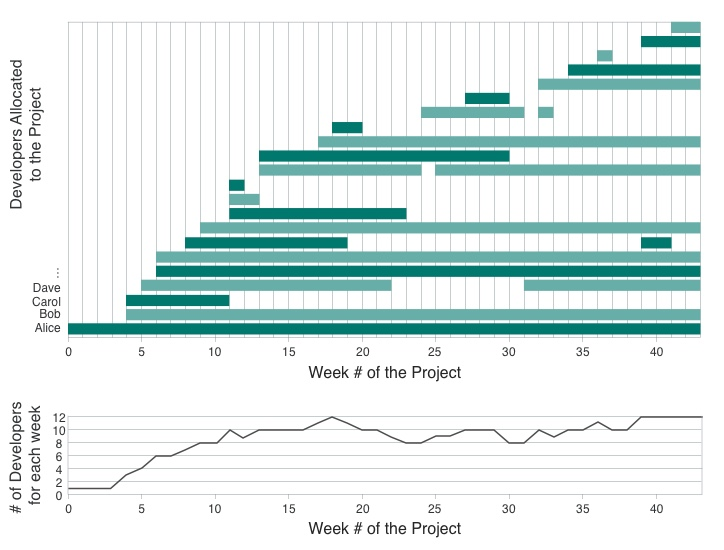
\includegraphics[width=7.1in]{DeveloperStaffing.jpg}
\caption{Developer Staffing}
\label{DeveloperStaffing}
\end{figure*}

Figure \ref{DeveloperStaffing} shows the staffing plan of the project. The bottom diagram shows the total number of developers allocated to the project at any given week. There is a steady ramp up from week 5 to week 12. The average number of developers assigned to the team is 9.8 and the maximum team size was 12 developers.

The top diagram shows that there were five developers who were on the project for most of its duration, that 22 people actually worked on the project, and that the maximum team size was 12 developers working together at the same time.

As a result of these rotations, the team did suffer a loss of sense of team. According to Tuckman's forming, storming, norming, and performing model \cite{TuckmanModel}, the team could not achieve a sense of identity as its member were routinely changing. 

Yet the team successfully completed the project while overcoming obstacles such as not having access to production back-end systems, not having access to expensive dependent physical components, and being slowed down to address cultural differences between Pivotal and the client's deployment organization. The client was extremely proud of the results. Regarding the first release, the client said that the team accomplished a multiple year project in 5 months. 

Conventional wisdom says that team churn is very disruptive for a team and should be avoided. Yet, Project Decem was able to succeed despite high team churn. This observation leads us to our first research question: \quotes{How does Pivotal overcome the team churn challenge in software development?}

\section{Theory of Sustainable Software Development}
\label{Theory}
This section could be structured as follows:
Theory brief overview???
RQ1: How does Pivotal overcome the team churn challenge in software development?
Practices
Synergy among practices [graph?]
RQ2: How developers feel about collective code ownership?
benefits
drawbacks / erosion
→ Tension

Sustainable Software Development is a collection of synergistic practices that enables the business entity to easily survive disruptions, such as vacations, terminations, rotation of team members, churn, or growing team size. It enables the engineering team to repeatedly deliver software features, even with complex systems or legacy code bases, resulting in throughput sustainability by establishing a software development culture where each developer is both empowered and enabled to modify any portion of the code base. As a result of implementing the theory, each engineer becomes replaceable, which ironically makes the team irreplaceable as it is performant and can handle challenging situations. 

The primary benefit to the employer is business agility. The engineering team continues to deliver software week after week, month after month, and survive cataclysmic events. Things do not fall apart when the superstar developer leaves. People can go on vacation whenever they need to because features or components are not critically tied to a particular individual. The team leverages the whole team's talents. This removes bottlenecks of \quotes{only Pat can work on these features.} Critical feature work can be parallelized since anyone can work on the feature, as opposed to an individual code owner. 

The primary benefit to the engineer team is the ability to work on every story, to understand the entire system, teaching opportunities to share one's expertise and to deeper learn subtle parts of the technologies. 

The primary cost is a shift from individual code ownership to collective code ownership. For some engineers, their sense of value and self-worth is derived from direct code ownership, and thus transitions to Sustainable Software Development should not be taken lightly. Sustainable Software Development works well with collaborative individuals and may not be suited for people who like to work on their own. Sustainable Software Development works when team members have the maturity to loosely hold temporary personal contributions understanding that the team may enhance any aspect of the product.

Sustainable Software Development is suited for companies that must routinely deliver value to their customers or stakeholders. Some companies are better positioned to withstand a quarter where nothing happens (from an external perspective) or  ``the forgotten two years of management waste” as described by one manager in this study. Hopefully, competitors have not caught up or surpassed the organization during the lost time. Both Pivotal Labs as a consulting practice and the growth of Pivotal's Cloud Foundry towards market dominance, depend on the continual development of features. Neither can afford to falter and both implement Sustainable Software Development.

Sustainable Software Development is that software development continues at a regular pace regardless of who is on the team, or rather regardless of changes in team composition.

\subsection{Research Question 1: How does Pivotal overcome the team churn challenge in software development?}
The synergy of the Sustainable Software Development practices is how Pivotal overcomes team churn.

<<explain synergy>>

Conventional wisdom says that team churn is very disruptive for a team and should be avoided. 
Pivotal views people rolling onto a project as an opportunity for the team to improve the current code base as they provide a new fresh perspective. They do not understand the code base and  reveal issues with code discoverability. They reveal the team's assumptions and challenge cargo culting. 

Rotating people onto a team will affect the team's sense of identity. Research shows that the Tuckman model may be restarted whatever the team composition changes. [Ref] Ironically, the team can continue to produce at a higher rate because of pair programming. A team that has been together for a while will develop patterns and habits corresponding to a high-performing team. Such as the emergence of nicknames or understanding each team member's little quirks. The team will learn each member strengths and how to utilize the strengths. 

Rotating people onto and off of project actually works even better if there is some continuity of people on the project.  On Project Decem, there were five developers from the beginning of the project to the end, with an additional 17 people who worked on the code base. For team with individual code ownership, this amount of churn probably would have been catastrophic. Because of the collective code ownership and the synergy between the practices, the team continued to deliver each week.

One of the concerns of individual code ownership is the team typically has a low Lottery Number, Bus Count, or Truck Number. These concepts capture the idea that people leaving a project can be very disruptive. Truck Number, \quotes{is the size of the smallest set of people in a project such that, if all of them got hit by a truck, the project would be in trouble.} \cite{WikiTruckNumber}. Rolling people off a project simulates a sequence of individual potentially catastrophic events.  A ten person team thriving despite 12 roll off events is remarkable. 

\subsection{Research Question 2: What practices enables the developers to modify any part of the code base?}
\subsubsection{Collective code ownership}
Collective code ownership is more than just a policy statement. The team saying \quotes{anyone can modify any piece the code} is not sufficient to achieve the desired results. It requires a corresponding set of related practices that must be in place to achieve collective code ownership. Thus collective code ownership is a dimension in which the team can have little or much ownership of the code. 

The sense of collective code ownership is not static. Project characteristics can actually erode the team's sense of ownership over the duration of a project. A team needs to counteract these erosions in order to increase their sense of ownership. Ownership is an emotional or qualitative attribute relating all the developers on the team to the project and the Code Base.

\strikeout{A team simply saying that they are adopting collective code ownership is not sufficient for them to achieve it, it needs to be coupled with practices.}

Removing collective code ownership makes sustainable software development challenging. Every line of code written via strong ownership is creating a knowledge silo. Code reviews is a mitigation strategy, but this increases the bus count to the reviewers, not the team. 

\subsubsection{Continuous refactorings and sustainable work pace}
The need for any pair to be able to work on any story results in continuous refactorings as a Sustainable Software Development practice. Taking the time to increase code discoverability, code readability, and code simplicity produces long term benefits. 

The current benefits from the continuous refactoring are actually enablements to help the team with collective code ownership. Code with poor discoverability, code that is hard to change decreases the team's sense of ownership.

There will be times where the team is tempted to incur technical debt, but these temptations should be resisted. One exception to this rule is when the business will not receive its next level of funding, or go out of business if the product is not shipped. Paying down any accrued technical debt immediately is required otherwise code apathy may set in. 

Sustainable work pace works hand in hand with continuous refactorings. If a team is asked to work additional time, that means the team is no longer able to manage up and is being pressured. During these stressful times it is critical for the team to double down on its practices and be more disciplined. Otherwise the team risks taking on technical debt. If the team is working overtime, sustainable development requires continuous refactorings. The team runs the risk that \quotes{refactoring later} turns into \quotes{refactoring never}

If a team is pressured to get their work done, then the team might focus on feature delivery at the expense of continuous refactorings. We saw this on Project Decem where the rush to get some features done, made it harder to maintain the code and thus decrease our ownership since we could no longer make easy modifications to parts of the code, we had to dig ourselves out to reclaim ownership of these areas.

In XP 2.0, Beck describes Energized Work as working only sustainable hours and resisting the urge to throw more time at a problem to regain control of a situation.  

A team working 90 hour work weeks can not claim to be business sustainable. 

Technical debt can lead to decreasing sense of collective code ownership, people do not like living in messy houses

The code does need constant tending (like a garden) and careful attention. Maybe stewardship.

Removing this practice produces the messy code. It is no longer easy for developers to work on any part of the code base.

If I'm listening to the code, and I see something really wrong, I should want to go fix it. If I have high \quotes{ownership} and feel like I'm a \quotes{caretaker} then I'll fix it. (Reminds me of conservation from Forestry, and stewardship.)

\subsubsection{Same work hours}
When the team arrives at the same time, the team can quickly rotate developers and form new pairs for the day. The evening becomes a natural interruption to the continuous software development workflow. Trying to schedule a time midday to rotate feels artificial, and even if the team says they will rotate later in the day, once pairs get into their stories and form context on what needs to be done, they typically forget about repairing until it it time to go home.

A team with flexible work hours will find it difficult to pair program on all stories. When developers arrive whenever they feel like it, the \quotes{rotating developers when context shared} practice becomes awkward. Assuming the team adopts core work hours, if someone consistently solos from 8 am to 10am, then they are building knowledge silos. Pivotal did try the experiment of pairing when developers arrived, but this meant that developers arriving early were making pairing decisions for the people who arrived later. A possible mitigation strategy would be soloing on simple clean-up chores and then switching to feature development when the whole team arrives. 

\subsubsection{Pair programming}
By pairing, two developers implement every feature. When the pairs rotate that knowledge is spread throughout the team and available to each new pair. 

Removing this practice results in solo programming where there is a clear owner for each commit. Research studies such as Birds are possible. It's easier for one developer to work on a track of work. In this situation, assigning stories to developers who have the least understanding about part of the code base forces knowledge sharing. This is a hard sell to management. Bird's study suggests this is one way to introduce defects. 

\subsubsection{Rotating developers when context shared}
Rotation of developers helps prevent knowledge silos from forming. We are trying to prevent the situation where to implement a story, I must pair with Rachel since she is the only person who understands how that part of the system works. Instead, we want the entire team to be able to modify the code. 

For a track of work, we want one developer to roll off and another developer to roll on.  We do not want one developer working on the same track for three days in a row. Likewise, if a story lasts longer than a day, then the developers need to rotate.

With any rule there are exceptions to this, this included. Maybe there is so much context needed to work on a story, that it would take a long time to bring a developer up to speed or the story does require deep technical expertise. In all of these cases be prepared with a mitigation strategy: schedule a team talk to expose people to that technology, use tri-programming to train two more developers on the technology. 

Whenever a knowledge silo begins to emerge, actively fight against it and spread that knowledge around. \quotes{Rachel really knows the Apple watch code base, we need her on that story or Zac knows the ins-and-outs of the siteminder integration, we need him to work on this} are signs that knowledge silos have emerged. 

Periodically there are stories that we find interesting and we want to work on them for a variety of reasons. Perhaps they use a technology that we know really well, or they involve a technology that we want to learn. Maybe we are fascinated by the feature set and we want to implement it. Maybe we like visual layout of a page. Maybe we love working on really challenging technical problems. Maybe we love routine and enjoy doing a story that has repetition in it. Whatever the reason, sometimes we want to \quotes{see it through} and we can express this desire in pair rotation. This request might be sourced/founded in personal ownership, and allowing it to happen may result in short term personal ownership. Allow a developer to carry on with a story is fine, but the team needs to be careful of a) creating knowledge silos (this can be solved by rotating the developer off of the story or having the team member share what they learned through a demo, code walk through or a team huddle. b) creating a sense of personal ownership.

If you remove this practice then developers can work on the same part of the code base, developing deep context, individual code ownership, and knowledge silos. With XP 1.0, and 2.0, it is possible for a developer to do this. 

Ideally developers work on the next, non-blocked story at the top of the backlog. When developers start skipping down the backlog, it is an indication that they might not have enough context to work on any story. On the example project, there was a knowledge silo about dealing with a bug with an obsolete technology that only a handful of people understood. Often developers would skip over stories and bugs related to that technology. At one point the product manager reminded the team to keep  \quotes{working from the top of backlog.}


\subsubsection{Test Driven Development, Behavior Driven Development}
The point is that every line of production code is tested before it is written.
In XP 1.0, Kent Beck describes this as simply \quotes{Testing} (automated unit tests) and in XP 2.0, Kent Beck describes this as \quotes{Test-first programming.} There is no good phrase to describe exactly what we do. It's a mash up of Test-Driven Development and Behavior Driven Development. While each project is different, programmers use BDD to describe interactions between the user and the system and use TDD at a unit test level. Both London School and Chicago School styles are employed with a slight bias towards contact testing using mocks as described by J. B. Rainsberger \cite{RainsbergerIntegrationTestsYouTube}

This creates a safety net for easy modification of tests, and empowers a pair to have the courage to make modifications to the code base. Without a test suite documenting the system specification, a strong code ownership model would probably be necessary.

In our ideal, the design emerges from the creation and exploration of the test cases.  

Removing testing results in developers no longer have the confidence to change the any part of the code without the concern of  breaking something else. A possible remedy is creating knowledge silos where developers own particular parts of the system and understand the ramifications of changes.

Removing this practice may results in the hard to change test code. Writing tests after implementation may result in false positive passing tests.

\subsubsection{Continuous Integration}
By continuous integration, we mean the practices espoused by XP 1.0 and 2.0, namely \quotes{Run tests before pushing code}, \quotes{Live on Master}, and \quotes{Promptly Fix Broken Builds}. Running a Continuous Integration box and having long running branches is an anti-pattern.

In order to remove the waste of merge conflicts, the entire team needs to be routinely merging their code onto master.  In an ideal flow, developers will merge their code to master many times a day. If a pair has not done merged to master by the afternoon, they typically start examining what about the nature of their work makes this difficult and is there a way to incrementally make these changes. Developers use branches to record spikes or to move code between machines during pairing rotation when the code is not ready for merging.  The anti-pattern is code that lives on only one machine for many days in a row. In this sense, the machine acts as a \quotes{virtual branch.} 

Why!!! If I have code only on my machine, no one else on the team can use or modify that code. If I know that people are \quotes{refactoring} a component for days, and they are asking the team not to touch certain classes to avoid merge conflicts, they are asserting exclusive ownership over the file. While this is a normal practice for a few hours, the team is losing collective ownership when it happens for a week. Pairs that work on that code and rotate out are not able to use any of the benefits of the work being done until it is merged back in. 

If you remove this practice then (just covered, reword here)

\subsubsection{Obtaining context}
This can happen by asking the team, asking a pair, remembering who did what at stand-up, looking through tracker to see who worked on a story. 2, 4, 6 person teams will have collective memory of who worked on which features. A 10 person team will need to be active in finding the answer to the question. Osmotic communication also helps when the person who worked on a story overhears another pair discussing a class.

While working on a story, a pair may discover that they are missing some key context that prevents them from efficiently proceeding. Instead of thrashing, it is common for the pair to interrupt another pair to gain the needed information. Thus interruptions are encouraged as it makes the entire team more efficient. How does the pair know who to interrupt? They rely on their awareness of who worked on each feature, or version control history will indicate who last worked on a software component. If the knowledge has left the team, then the pair will need to dig into the code to understand what is going on. It is necessary work and at the end, two team members will now have that knowledge to share with the team. 

In Chong's ethnographic study of an Extreme Programming team compared to a traditional team \cite{ChongNominum}, she observed that ``transmission of awareness information is a relatively effortless act in the XP environment” as is consistent with teams that work in highly collaborative work. 

Removing this practice means that people would need to relearn the context and answering questions such as \quotes{what is the code doing?}, \quotes{why was it built this way?}, and \quotes{what are the business concerns?}. On a small scale, it just unnecessary waste. On a large scale, this is the problem we are trying to solve.
\subsection{Synergy}

Others have attempted to achieve collective code ownership in industry, but as soon as one removes one of the practices and other results are less interesting. For example replacement pair programming with solo programming, now requires the team to jump through new hoops. For example, when working on the next story for the registration feature, that story should be assigned to the developer who has worked on it the least recently, as they will have the lease context and will verify quickly how easy the code is to work with. This practice is a hard sell for management, and may be less effective than Sustainable Software Development.
\section{Collective Code Ownership}
\label{CollectiveCodeOwnership}

Software development happens by people, and we need to factor psychological considerations. As one engineer expressed, \quotes{we are people} and our interactions with the code is as meaningful as the code itself. Listening, caring, and empathy for one another allows the team to work through differences of opinion towards a better than imagined code base. As one designer said, \quotes{you have to be an adult to work here.} Letting go of personal ownership enables the team to achieve results only achievable by the team. In need, Sustainable Software Development fosters an environment where the whole is more than the sum of the parts. 
\subsection{Research Question 3: What negatively affects the developers' sense of collective code ownership?}
\subsubsection{Increasing Team Size}

The primary researcher participated on teams of size 2, 4, 6, 6, and 10, and observed that as the team size increases, the ability to have context on the system decreases. Each day the other pairs are adding to the system. On a five pair team, so much work is happening each day that it is hard to keep track of everything that changes.

One developer on a 10 person project said, \quotes{I feel that we don't have that context spread around fully but then again having five, sometimes six pairs on the project makes it go really fast so it's hard to keep context….it's a big team and you can be working on one track for a week perhaps and then the other four pairs like we move fast like things just change under you and you get back to some other place and you're like oh what happened here.  So because of that speed, it's harder to keep context on everything.}

As a coping strategy, a different developer on that project, before the work day started, would skim the git commits from the previous day to learn about new classes, changes in design, and understand what features were added. As a possible mitigation strategy, each pair of the entire team could start their pairing day by reviewing changes from the previous day. It's additional work, a form of waste, and thus one of the costs of a large team. 

When developers do not have context about part of a system, or context about what remains to be done to finish a story, reluctance to start the next at the top of the backlog emerges, they would rather take a story that touches part of the system that they know. As a third developer reflected, Quote: \quotes{It does make me not completely comfortable to jump into stories on certain aspects.}

As team size increases, there is a potential risk of isolating each individual developer from a sense of code ownership. 

\strikeout{A greenfield project typically starts with one pair laying down the \quotes{plumbing} of the new system by performing tasks such as setting up dev machines with common development environment, initializing the code base, adding just enough frameworks to get running code, and setting up continuous integration with automatic deployment to an acceptance environment. If the desired team size is six developers, the remaining four developers would be added after inception (kickoff) meeting. For a larger team, developers will be added incrementally depending on the needs of a project. Some clients want to minimize burn rate by being as efficient as possible with developer resources whereas other clients want to deliver the maximum number of features by a certain point in time and are willing to have extra developers on a team even though it's less efficient.}

\subsubsection{ Deprioritizing continuous refactoring resulting in increasing code apathy  }

When developers are pressured to deliver more features at the expense of continuous refactoring, then the code acquires technical debt, the code is harder to work with, and developers can become apathetic about the code. When developers begin to feel code apathy, this decreases their sense of code ownership. Most stories typically involve some refactoring, as developers are encouraged to make the code's design cleaner, easier to understand, and easier to find the component associated with its responsibility. (It's preferred to do pre-refactorings of doing complicated work to make the implementation of the current story as simple and easy as possible.) When refactoring is skipped that means code was simply bolted on to the existing design. Each time the team bolts something else on, it gets harder to bolt on something else. Thus, a dilemma arises for the programmers working on the next story to touch this part of the code: do they continue bolting on more code, or do they perform the pretermitted refactoring. When the team begins avoiding refactorings, it's a sign that code apathy may be settling in. Developers caring less about the craftsmanship of the code reflects a growing code apathy. 

One developer feels \quotes{proud and disgusted} about the code base. He is simultaneously proud of each refactoring that the team performed and disgusted by the technical debt the team accrued by taking shortcuts to ship more features. 

Before the first launch of Project Decem, the product manager suggested that the team deliver more features at the cost of tech debt. For some of the team, this was an unacceptable tradeoff, and decided not to cut corners. Others on the team did choose technical debt, and the entire team ended up paying for the consequences by extensive refactors after the launch. On a team communal code base, one pair adding tech debt affects everyone on the team

The team wants to feel a \quotes{pride of improving code quality}.  It feels good to be improving the code design and readability. If the team starts neglecting these items, it can create a sense of disgust, and an apathy of the code can spread throughout out the team.

\subsubsection{Increasing Feature Apathy}
Feature apathy is when a developer begins to not care about the product of the features he is working on. When a developer feels like their voice isn't heard in the product feature set, then they can be less motivated to work on the project. Part of our balanced team approach is collaboration, and when product isn't listening to feedback from their developers, then the developers might feel less ownership of the product.

\subsubsection{Increasing Team Apathy}
Team Apathy is when a developer does not feel apart of the team. When this occurs it can be hard to feel collective ownership of the code base when one doesn't feel part of the collective.

When a developer begins to feel that the team doesn't care about them, the developer can begin to care less about the success of the project and the quality of the code base. Identified behaviors include feeling unheard by the team, team members interrupting them during discussions, or talking beyond their level of technical expertise. One developer is a visual learner and the team talked about code but never looked at code during team discussions. It was hard for the developer to follow discussions about code when the developer hadn't seen in awhile or an example or participate in conversations about coding practices when examples without seeing a concrete example of the issue. When the developer brought this issue to the team, but the team continued with the status quo, the developer felt marginalized by the team.

As another developer expressed, \quotes{not listening to each other can create apathy.}

When apathy settles in, team members may result in expecting someone else will solve the problem. Given the technical complexity of the product sometimes the next story on the backlog would be blocked. Instead of proactively working with product, one developer adopted the attitude \quotes{Well, this [story] is blocked and it's somebody else's problem.} 

When picking up a story, it is the developer's responsibility to verify that the story contains clear acceptance criteria. If it doesn't, conversations with product are necessary. This same developer recalled \quotes{In this case, I don't feel like spending the extra energy to go and say, `Hey, are you sure? Is this what you want?'} Apathy can result in a less than perfect product.

\subsubsection{Poor onboarding of developers}
Poor onboarding of developers is one way for developers to not feel part of the team and thus not feel much sense of code ownership. On one project, there was a time pressure crunch and the team was feeling the pressure to deliver stories. When some people were added, it was a \quotes{sink or swim} attitude. For example, the person was left to solo for the first couple of hours. While we shouldn't have to coddle a developer, the personal touch can go a long way. If someone doesn't feel part of the team, how can they feel ownership of the code base?  Spending some extra time when a person rolls onto a project pays dividends. 

\subsubsection{Decreasing quality}
A product suffering from quality issues threatens the an individual's sense of ownership. First, an engineer may not want to be identified with that product internally or externally to the company.  Second,  developers need a balance of feature work and bug fixing each week. Working only on bugs for weeks will affect a sense of ownership.    
 
\subsubsection{Not understanding the system}
An engineer does not understand the system decreases a sense of ownership. 

\subsubsection{Breakdowns in pair programming }
When the pairing experience breaks down, individual code ownership can replace collective code ownership.  One developer reflected about one particular situation where their pair took over and ignored their input, \quotes{I did not understand what was really going on. I wouldn't be able to deeply explain it. I wouldn't be able to maintain it. I didn't really write it, so i feel very little ownership of it.} We call this  \quotes{performance pair programming} when one developer plows through a story, stops listening to their pair. Ideally pair programming is a collaborative experience where both individuals can't tell who wrote what code. 

In our research we identified many ways in which a team may decrease its sense of collective code ownership.
\subsection{Research Question 4: What are the downsides of collective code ownership?}
\subsubsection{Unknowingly working on dangerous parts of code}
Although not directly observed during this research study, it is possible for a pair of developers to naively work on code that is potentially very dangerous to modify. While this is a concern too with individual code ownership, presumably those files would be owned by a subject matter expert. Ironically, it seems that cross training would be very important and enabling everyone on the team to understand the dangers would be important if the the subject matter were to leave the team.  

We did observed pairs asking others for context and help, and that interaction would be one way to warn pairs about subtle problems. Another potential solution is to clearly document that \quotes{there be dragons here.} 

\subsubsection{Transitioning to Collective Code Ownership}
For some individuals, their sense of value, worth, and identity are derived from what they produce. Since Sustainable Software Development requires a shift from individual ownership to collective ownership, the transition should not be taken lightly as we are asking them to shift how they value and perceive themselves. 

A recent hire to Pivotal described his initial experience as \quotes{seeing my work slowly removed from app}. When reflecting on the daily rotation, this developer recalled occasions of wanting to hang onto the work.  His attitude of \quotes{I want to see it through} evolved into \quotes{someone else is going to take over and they're going to do fine. I can move onto something else and that's okay} The developer learned the rhythm of story rotation and developed the trust that the rest of the team will do a good job. Developers rolling off a story in flight can look in anticipation to see what the next pair produces and see how they solved the problem. 
Eventually, team members recognize the lack of long term individual authorship, learn to expect their code to be transitory, and thus loosely hold personal contributions. \quotes{The code that I write today may be in the code base for a little while but will evolve into something better.}  

Some developers immediately see the benefits of being able to modify any part of the code base and quickly shift from \quotes{I made this} (personal ownership) to \quotes{we made this.} 

\strikeout{One might argue that all software development is transitory, and that the code we write today will be replaced by something else in the future. Yet the illusion of personal ownership is strong, and needs consideration. Since the code is owned by a company, the perception of both \quotes{collective ownership} or \quotes{personal ownership} is an illusion. It is not personal property or private property. Yet the illusion is powerful and seductive. A manager doesn't own his team or his office, yet the trappings of management are strong.}

The developer transitions from owner to stewards and caretakers. Here one Pivot was struggling to describe their relationship with the code on a very challenging project and settled in on the caretaker metaphor : \quotes{Sometimes I kind of feel like a janitor to it.  Maybe caretaker would be better.  Yeah, probably caretaker. I feel like a janitor just cleans up messes but a caretaker like also makes things better.}

Our ability to control something influences our sense of ownership, and ownership influences our sense of identity. 

For someone transitioning to collective code ownership with strong individual ownership tendencies, we recommend starting that person on a four person team. This will allow the person to see the benefits of shared code ownership while slowly practicing releasing individual ownership. On a four person team, each daily rotation creates pairs with full knowledge of what happened yesterday.  

Here is an example pairing rotation illustrating that each day, the new pairs have full context about yesterday's changes:
\texttt{
Day 1: A B, C D,
Day 2: A C, B D,
Day 3: A D, B C
}

We suspect that improv games and other collaboration games can help teams see the benefits of collective code ownership and practice the skills of letting go of control expectations while learning to be pleasantly surprised by what emerges.

When a team achieves a sense of collective ownership, the magic happens: \quotes{people are a lot more flexible all across the board with the changing things or accepting feedback or collaborating} and \quotes{we want the best possible product that's best for users … we just want the best thing out there.} Then the team can say \quotes{hey this is our code.}
\section{Theory Evaluation}
\label{TheoryEvaluation}

In assessing a Grounded Theory research study, Charmaz identifies four criteria for evaluating a grounded theory study: credibility, (\quotes{is there sufficient data}), originality, (\quotes{do the categories offer new insights}), resonance (\quotes{does the theory make sense to participants}), usefulness (\quotes{does the theory offer useful interpretations}) \cite{StolGTinSE}. 

\begin{itemize}
\item 
\textbf{credibility:}  The number of open ended interviews and the field notes from participant observation serve as a rich data set for the analysis. The developer staffing for the project serves as a compelling illustration of the theory in practice

\item
\textbf{originality:} Many of the practices of Sustainable Software Development are defined in Extreme Programming, this is not surprising as the subject under study practices Extreme Programming. Three things make this work original. First, several of the practices are not listed in Extreme Programming and are crucial to the success of Sustainable Software Development theory at Pivotal. Some of these practices are not followed at other Extreme Programming companies such as Extreme Labs. Second, this work packages these ideas into a coherent whole and helps distill the technical practices of Extreme Programming into a one key category. Third, this study provides the first concrete example of collective code ownership enabling a high rotation of developers through a team (when it is combined with the other practices of the theory.)

\item
\textbf{resonance:} When shown to participants, they immediately understand the theory and want to understand the nuances of erosion.

\item
\textbf{usefulness:} 
On tours with where potential clients see how Pivotal builds software, the theory succinctly describes Pivotal how many of the practices simultaneously achieves the business goals of the client and Pivotal. The theory better informs pivots as to why we purposefully avoid knowledge silos and gives an argument for the strong cohesion of the theory's practices and why those should be incorporated together without taylorization. 
\end{itemize}

\section{Threats to Validity}

External Validity. Generalizability across situations: a limitation of grounded theory is that the theory emerges from a particular context and may not be applicable to other situations. This work analyzed software projects at the Silicon Valley office of Pivotal following Extreme Programming. The results might not be applicable to other teams in industry wanting collective code ownership or  following Extreme Programming. Replicating the results with other teams would mitigate this threat.

Internal Validity. Researcher bias: a risk of the participant-observer technique is that the researcher may lose perspective and become biased by being a member of the team. An outside observer might see something the researcher missed. We mitigated this risk with recorded interviews and a colleague review of the coding process. 

Prior knowledge bias: With grounded theory prior knowledge can aid the researcher in looking at interesting research questions or create difficulties in blinding the researcher about possible explanations. \cite{GlaserIssues}. This work leverages the rich history of Extreme Programming, and the theory refines core aspects of Extreme Programming. 

Reword this to be a limitation: ``Identity" and ``etiquette" may affect what participants may reveal. Identity refers to the relationship of the researcher and the participant. For example, a professor interviewing students about learning techniques. Different kinds of strategies can be employed. A researcher could distancing oneself from positions of authority: a professor could interview students in a different degree program. To alter power imbalance, a domain expert researcher might offer ``personal and professional views to encourage reciprocity." Etiquette refers to social norms and customs. Participants might not want to reveal information to a stranger. A company rule of secrecy might make it difficult for a researcher to get the needed information. Framing questions is one way to elicit this kind of information. ``Some people have mentioned having negative pair programming sessions. Has that happened to you?" 


If one wants to achieve collective code ownership, it would be dangerous to pick and choose part of the practices of Sustainable Software Development. If one wants to achieve collective code owne

There theoretically might be other ways to achieve collective code ownership, as defined in this paper. However, 

\section{Future Research}
Developers are driven by code craftsmanship. Designers are driven by usability of features and aesthetics, aspects that reflect on their talents and training. What drives ownership for product managers? All seem to care about whether any one will actually use the product and whether their work actually matters. In future work,  we plan to examine how ownership is driven by different factors for designers, developers, and product managers.

Some programmers naturally adapt to collective code ownership, while others struggle with the transition. In future research we would follow new Pivotal engineers and examine their journey in transitioning from individual code ownership to collective code ownership. Perhaps there are 
specific practices that Pivotal or the development team could employ ease the transition. 

How does rolling on and off for short durations affect the sense of collective code ownership? We plan to interview people who join a project for a week or two. 



Further research is necessary to determine the optimal team size for collective code ownership. Early indications suggest that a four person team is a sweet spot for introducing Sustainable Software Development. With a four person team of two pairs, each day one developer is working on half of the new feature development. When they rotate the next day, each developer will be paired with a developer from the other pair. Each new pair will have the entire knowledge of what happened yesterday. 


\section{Conclusions}

\section{Find a Home}

With a team of 10 or less, if there are uniform commits per dev per file, then the percentage commits per dev per file is 10% which is strong ownership according to Bird.

http://guide.agilealliance.org/guide/cco.html  
http://swreflections.blogspot.com/2013/04/code-ownership-who-should-own-code.html
http://martinfowler.com/bliki/ShiftingToCodeOwnership.html
http://c2.com/cgi/wiki?CodeOwnership
http://research.microsoft.com/pubs/140711/ownership.pdf

I noticed that my sense of ownership increased after I started showing the application to other people.



\section{Remove me}
\subsection{Research Objective}
The methodology under study is Extreme Programming. \cite{ExtremeProgramming2004} Pivotal Labs has used Extreme Programming since the late 1990s to enable collaborative experiences for Pivotal Labs clients.


Research Question 1: What is fundamental to software development as it is done at Pivotal? 

Research Question 2: How do the practices support Sustainable Software Development? 

Research Question 3: What can negatively affect Sustainable Software Development?





